\documentclass{beamer}

\usepackage{amsmath,amssymb,amsfonts}
\usepackage{bibentry}
\usepackage{graphicx}
\usepackage{listings}

\lstdefinelanguage{GF}{
    morekeywords={ abstract, concrete, resource, interface, instance,
        incomplete, of, with, open,
        cat, fun, lincat, lin, oper, flags, param
    },
    morecomment=[l]{--},
    morecomment=[s]{\{-}{-\}},
    morestring=[b]",
    basicstyle=\footnotesize
}

\lstdefinelanguage{GFcmd}{
    morekeywords={parse, linearize, view_tree},
    morestring=[b]",
    basicstyle=\footnotesize
}

\title{Using GF for Math Linguistics}   
\author{Jan Frederik Schaefer} 
\date{\today} 

\usetheme{Pittsburgh}
\usecolortheme{beaver}

\begin{document}

\frame{\titlepage} 

\section{Introduction}

\frame{
    \frametitle{GF - Grammatical Framework}
    \begin{itemize}
        \item ``A programming language for multilingual grammar applications''
        \item Natural language as formal language $\Rightarrow$ limited coverage but high precision
    \end{itemize}
}

\section{Introductory Examples}

\frame{
    \frametitle{First Example - Abstract Grammar}

    \lstinputlisting[language=GF]{gf/One.gf}

    \vspace{1em}
    Example tree: \lstinline[language=GFcmd]{And (Loves John Mary) (Loves John John)}

    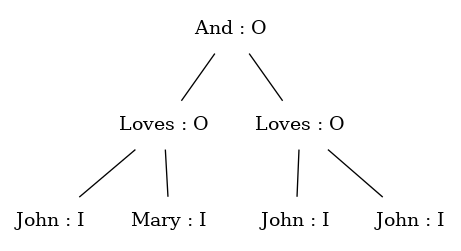
\includegraphics[scale=0.3]{graph_1.png}
}

\begin{frame}[fragile]
    \frametitle{First Example - Concrete English Grammar}

    \lstinputlisting[language=GF]{gf/OneEng.gf}

    \vspace{2em}
\begin{lstlisting}[language=GFcmd, breaklines=true]
> linearize And (Loves John Mary) (Loves John John)
John loves Mary and John loves John
\end{lstlisting}
\end{frame}

\begin{frame}[fragile]
    \frametitle{First Example - Concrete German Grammar}

    \lstinputlisting[language=GF]{gf/OneGer.gf}

    \vspace{2em}
\begin{lstlisting}[language=GFcmd, breaklines=true]
> linearize -lang=Ger And (Loves John Mary) (Loves John John)
Johann liebt Marie und Johann liebt Johann
\end{lstlisting}
\end{frame}

\begin{frame}[fragile]
    \frametitle{First Example - Translation}
\begin{lstlisting}[language=GFcmd, breaklines=true]
> parse -lang=Ger -cat=O "Johannes liebt Maria und Johannes liebt Johannes"
And (Loves John Mary) (Loves John John)

> parse -lang=Ger -cat=O "Johannes liebt Maria und Johannes liebt Johannes" | view_tree
\end{lstlisting}
    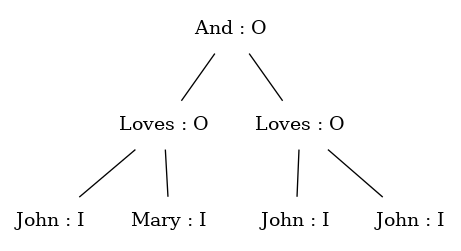
\includegraphics[scale=0.3]{graph_1.png}
\begin{lstlisting}[language=GFcmd, breaklines=true]
> parse -lang=Ger -cat=O "Johannes liebt Maria und Johannes liebt Johannes" | linearize -lang=Eng
John loves Mary and John loves John
\end{lstlisting}
\end{frame}

\section{The Resource Grammar}

\begin{frame}[fragile]
    \frametitle{Using the Resource Grammar - Abstract Grammar}

    \lstinputlisting[language=GF]{gf/Two.gf}

    \vspace{2em}
    Challenge: \lstinline[language=GFcmd]{Loves (And_I John Mary) John}
    
    \vspace{1em}
    \emph{$\leadsto$ The ending of the verb depends on the subject}
\end{frame}

\begin{frame}[fragile]
    \frametitle{Using the Resource Grammar - Concrete English Grammar}

    \lstinputlisting[language=GF]{gf/TwoEng.gf}

    \vspace{1em}
    The resource grammar takes care of that for us:
    % We can use the resource grammar to avoid dealing with grammatical subtleties ourselves.
\begin{lstlisting}[language=GFcmd, breaklines=true]
> linearize Loves Mary John
Mary loves John

> linearize Loves (And_I John Mary) John
John and Mary love John
\end{lstlisting}
\end{frame}

\begin{frame}[fragile]
    \frametitle{Using the Resource Grammar - Semantic vs Syntactic}
    \begin{minipage}{0.31\textwidth}
        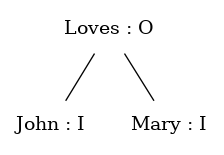
\includegraphics[width=1.1\textwidth]{jlm_sem.png}
    \end{minipage}
    \begin{minipage}{0.64\textwidth}
        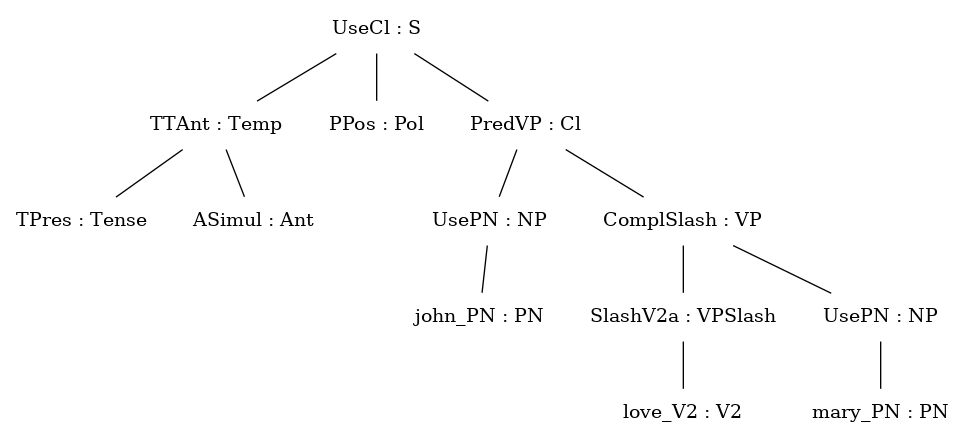
\includegraphics[width=1.1\textwidth]{jlm_syn.png}
    \end{minipage}


\end{frame}

\begin{frame}[fragile]
    \frametitle{Record Types}
\begin{lstlisting}[language=GF, breaklines=true]
lincat
    NP = {s : NPCase => Str ; a : Agr} ;

param
    Number = Sg | Pl ;
    Gender = Neutr | Masc | Fem ;
    Agr = AgP1 Number | AgP2 Number | AgP3Sg Gender | AgP3Pl Gender ;
\end{lstlisting}
\end{frame}

\begin{frame}[fragile]
    \frametitle{Operations}
\begin{lstlisting}[language=GF, breaklines=true]
lin
    UsePN pn = {s = \\c => pn.s ! npcase2case c ; a = agrgP3 Sg pn.g} ; 

oper
    mkNP : PN -> NP = UsePN;
         -- eta reduction of \pn -> UsePN pn
\end{lstlisting}
\end{frame}




\end{document}
